\documentclass[12pt, legalpaper]{exam}
\usepackage[utf8]{inputenc}
\usepackage[english]{babel}
\usepackage[margin=.8in]{geometry}
\usepackage{amsmath,amssymb}
\usepackage{multicol}
\usepackage{graphicx}
\usepackage{tikz}
\usepackage{lastpage}
\usepackage{tabularx}
\usepackage{hyperref}
\usepackage{tcolorbox}
\newcommand{\course}{Introduction to Optimization}
\newcommand{\term}{Fall 2023}
\newcommand{\examnum}{Report of Programming Task 1}


\usepackage{listings}

\begin{document}
\noindent \examnum \, of the  course ''\course'' - \term


\noindent
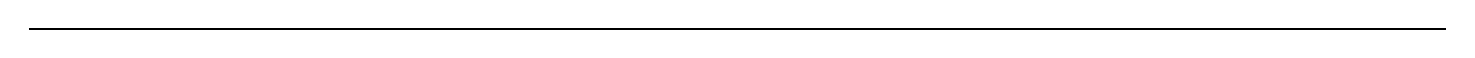
\begin{tikzpicture}
\draw[thick] (0,0) -- (18,0);
\end{tikzpicture}




\vspace{12pt}
\begin{center}
    \textbf{Report 1}
\end{center}
% \noindent \textbf{Requirements}

\vspace{12pt}

\noindent  \textbf{Team information.}

\begin{itemize}
    \item Team leader: Aleksandr Ryabov
    \item Team member 1: Aleksandr Ryabov
    \item Team member 2: Aleksandr Ryabov
    \item Team member 3: Aleksandr Ryabov
    \item Team member 4: Aleksandr Ryabov
    \item Team member 5: Aleksandr Ryabov
\end{itemize}
\vspace{12pt}
\noindent     \textbf{Link to the product.}
\begin{itemize}
    \item The product is available:  
\end{itemize}

\vspace{12pt}

\noindent  \textbf{Programming language.}
\begin{itemize}
    \item Programming language: Python
\end{itemize}

\vspace{12pt}

\noindent  \textbf{Linear programming problem.}
\begin{itemize}
\item Maximization or Minimization?
\\
Programm can solve both types of LPP. 
\vspace{10pt}
    \item Objective function: $F = 5x_1 + 4x_2 + 0x_3 + 0x_4 + 0x_5 + 0x_6$
    \vspace{10pt}
    \item Constraint functions:
    \begin{gather*}
        6x_1 + 4x_2 + x_3 = 24 \\
        1x_1 + 2x_2 + x_4 = 6  \\
        -1x_1 + 1x_2 + x_5 = 1 \\
        0x_1 + 1x_2 + x_6 = 2  \\
        x_1,...,x_6 \geq 0
    \end{gather*}

\end{itemize}



\noindent     \textbf{Input}

\vspace{12pt}
The input contains:
\begin{itemize}
    \item Maximization or minimization problem
    \item A vector of coefficients of objective function - $A$.
    \item Size of the matrix of coefficients of constraint function - $m$ and $n$
    \item A matrix of coefficients of constraint function - $C$.
    \item A vector of right-hand side numbers - $b$.
    \item The approximation accuracy $approx$.
\end{itemize}

\vspace{12pt}
\textbf{Example of input:}
\begin{verbatim}
    1 
    
    5  4  0  0  0  0

    4  6

    6  4  1  0  0  0 
    1  2  0  1  0  0
    -1 1  0  0  1  0
    0  1  0  0  0  1

    24  6  1  2

    1.0000001
\end{verbatim}

\vspace{12pt}
\noindent     \textbf{Output/Results}

The output contains:
\begin{itemize}
    \item Messange with error and string "The method is not applicable!"
    
or
    \item Messange with programm success
    \item A vector of decision variables - $X^*$.
    \item Maximum (minimum) value of the objective function.
\end{itemize}

\vspace{12pt}
\textbf{Example of output:}

\begin{verbatim}
    ### Maximum achived ###

    ######################################
    ### ANSWER                         ###
    ### Vector of decision variables   ###
    ### Values of 'x' vector is [3.0, 1.5, 0, 0, 2.5, 0.5]
    ### Value of function is 21
    ### Programm finished successfully ###
    ######################################
\end{verbatim}

\noindent
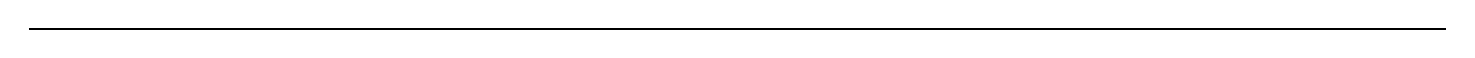
\begin{tikzpicture}
\draw[thick] (0,0) -- (18,0);
\end{tikzpicture}




\vspace{24pt}
\noindent     \textbf{Code of the program:}


\begin{lstlisting}{Python}
    import numpy as np
    import itertools as itls
    import math
    from decimal import Decimal
    
    # Disable 'divide by zero' warning
    np.seterr(divide='ignore')  
    
    # Welcoming
    print("### Welcome to Simplex method programm *_* ")
    
    # Read input values
    print("### Is your linear program about maximization?")
    maximization = bool(int(
        input("### If yes, print 1, else print 0: ")))
    
    temp_str = str(input(
    "### Write a vector of coefficients of objective function: \n"))
    A = np.array(list(map(float, temp_str.split())), np.float64)
    
    a, b = map(int, 
    input("### Write size of the matrix m and n: ").split())
    print("### Write a matrix of 
        coefficients of constraint function: ")
    
    arr = []
    for _ in range(a):
        temp_str = str(input())
        arr.append(list(map(float, temp_str.split())))
    
    C = np.array(arr, np.float64)
    
    temp_str = str(
        input("### Write a vector of right-hand side numbers: \n"))
    b = np.array(list(map(float, temp_str.split())), np.float64)
    
    approx = Decimal(input("### Write approximation accuracy: "))
    approx = abs(approx.as_tuple().exponent)
    
    # Set up presicion
    # np.set_printoptions(precision=approx, suppress=True)
    
    # Save shape of array 
    n, m = C.shape
    
    # Step 0
    # Find basic feasible solution
    
    # Iterate over all possible variance of 
    # basic and non-basic variables (vectors)
    for seq in itls.permutations(((m - n) * [0] + n * [1]), m):
    
        # Generate index sequence for array shaping
        basic_seq = [i for i in range(0, len(seq)) if seq[i] == 1]
        non_basic_seq = [i for i in range(0, len(seq)) if seq[i] == 0]
    
        # Check linear dependency 
        # using eigenvalue decomposition 
        lambdas, V = np.linalg.eig(C[:, basic_seq].T)
        
        # If vectors are linear dependent,
        # trying to find other
        # else start simplex algorithm 
        if len(C[:, basic_seq][lambdas == 0, :]) != 0 :
            continue
        else:
            break 
    
    while True:
        
        # Step 1 & 2
        # Compute inverse and z - c
        # Check optimality of the solution
    
        # Count X_b
        X_b = np.linalg.inv(C[:, basic_seq]) @ b
    
        # Count z - c        
        Z_c = A[basic_seq] @ np.linalg.inv(C[:, basic_seq]) \
                @ C[:, non_basic_seq] - A[non_basic_seq]
    
        # Count z
        z = A[basic_seq] @ X_b
    
        # Cheking optimality of the solution
    
        # Maximization optimal
        if (maximization and all(i > 0 for i in Z_c)):
            print("### Maximum achived ###")
            break
    
        # Minimazation optimal
        elif (not maximization and all(i <= 0 for i in Z_c)):
            print("### Minimum achived ###")
            break
            
        # Min/Max not optimal
        else:
    
            # Determine entering variable (vector)
            enter_var_ind = 0
            if maximization:
                enter_var_ind = np.argmin(Z_c)
            else: 
                enter_var_ind = np.argmax(Z_c)
    
    
            # Step 3
            # Check solition bound
            # Determine leaving variable (vector)
    
            # Count B_p
            B_p = np.linalg.inv(C[:, basic_seq]) @ C[:, enter_var_ind]
    
            # Check solution bound
            if all(i <= 0 for i in B_p):
                print("### Solution is unbounded ###")
                print("### Exit from programm ###")
                exit()
    
            # Compute slope cooficient
            k = np.divide(X_b, B_p)
            k = [i if (i >= 0 and i != float('inf')) 
                    else float('inf') for i in k]
    
            # Determine leaving value
            leaving_var_ind = np.argmin(k)
    
    
            # Step 4
            # Form new basis
    
            # Update state of the basic and non-basic vectors
            non_basic_seq[enter_var_ind], basic_seq[leaving_var_ind] \
            = basic_seq[leaving_var_ind], non_basic_seq[enter_var_ind]
    
    # Final vector x generation
    X_final = [round(X_b[basic_seq.index(i)], approx)
                 if i in basic_seq else 0 for i in range(m)]
    
    # Answer output
    print()
    print("######################################")
    print("### ANSWER                         ###")
    print("### Vector of decision variables   ###")
    print("### Values of 'x' vector is", X_final)
    print("### Value of function is", math.ceil(z))
    print("### Programm finished successfully ###")
    print("######################################")
    
\end{lstlisting}

\end{document}
